\documentclass[a4paper,12pt]{article}
\usepackage[utf8]{inputenc}
\usepackage[spanish]{babel}
\usepackage{color}
\usepackage{parskip}
\usepackage{graphicx}
\usepackage{multirow}
\usepackage{listings}
\usepackage{vmargin}
\graphicspath{ {imagenes/} }
\definecolor{mygreen}{rgb}{0,0.6,0}
\definecolor{lbcolor}{rgb}{0.9,0.9,0.9}
\usepackage{epstopdf}


\setpapersize{A4}
\setmargins{2.5cm}       % margen izquierdo
{1.5cm}                        % margen superior
{16.5cm}                      % anchura del texto
{23.42cm}                    % altura del texto
{10pt}                           % altura de los encabezados
{1cm}                           % espacio entre el texto y los encabezados
{0pt}                             % altura del pie de página
{2cm}     

\lstset{
backgroundcolor=\color{lbcolor},
    tabsize=4,    
%   rulecolor=,
    language=[GNU]C++,
        basicstyle=\tiny,
        aboveskip={1.5\baselineskip},
        columns=fixed,
        showstringspaces=false,
        extendedchars=false,
        breaklines=true,
        prebreak = \raisebox{0ex}[0ex][0ex]{\ensuremath{\hookleftarrow}},
        frame=single,
        showtabs=false,
        showspaces=false,
        showstringspaces=false,
        identifierstyle=\ttfamily,
        keywordstyle=\color[rgb]{0,0,1},
        commentstyle=\color[rgb]{0.026,0.112,0.095},
        stringstyle=\color{red},
        numberstyle=\color[rgb]{0.205, 0.142, 0.73},
%        \lstdefinestyle{C++}{language=C++,style=numbers}’.
}

\begin{document}
   \section{Problema}
   Desarrollar un paqute de software que genere automaticamente analizadores sintacticos para lenguajes regulares. En primer lugar, escriban un programa que acepte gramaticas regulares como entrada y genere como salidas las tablas de transiciones correspondientes. Luego escriba un programa que analice su cadena de entrada de acuerdo con la tabla de transiciones generada por el programa anterior.
   \section{Código}
    \subsection{GramaticaRegular.h}
      \begin{lstlisting}
#ifndef GRAMATICAREGULAR_H
#define GRAMATICAREGULAR_H
#include <fstream>
#include <iostream>
#include <map>
#include "fstream"

using namespace std;

class GramaticaRegular
{
    public:
        GramaticaRegular();
        GramaticaRegular(string file);
        void imprimirTabla();
        void generarAutomata();
        bool reconocerCadena(string);
        virtual ~GramaticaRegular();
    protected:
    private:
     map<char,map<char,char>> tablaDeTransiciones;
     char estadoInicial;
};

bool GramaticaRegular::reconocerCadena(string file){
    ifstream archivo(file.c_str());
    if(archivo.fail()){
	cout<<"El archivo "<<file<< "no se puede abrir o no existe"<<endl; 
	return false;
    }
    char cad[128];
    archivo.getline(cad,128);
    string cadena(cad);
    char estadoActual = estadoInicial;
    for(auto iter = cadena.begin(); iter != cadena.end(); ++iter){
        if(estadoActual == '#') return false;
        if(tablaDeTransiciones.begin()->second.find(*iter) != tablaDeTransiciones.begin()->second.end()){
            estadoActual = tablaDeTransiciones[estadoActual][*iter];
        }
        else return false;
    }
    if(tablaDeTransiciones[estadoActual]['%'] == '$')return true;
    return false;
}

void GramaticaRegular::generarAutomata(){
    ofstream archivo("eje.dot");
    char es = estadoInicial;
    archivo<<"digraph{"<<endl;
    for(auto iter = tablaDeTransiciones.begin(); iter != tablaDeTransiciones.end(); ++iter){
        for(auto iter2 = iter->second.begin(); iter2 != iter->second.end(); ++iter2){
            if(iter2->first != '%'){
                if(iter2->second != '#'){
                    archivo<<iter->first<<"->"<<iter2->second<<"[label =\""<<iter2->first<<"\"];"<<endl;
                }
            }
            else{
                if(iter2->second == '$'){
                    if(iter->first == estadoInicial) archivo<<iter->first<<" [color = \"blue\"];"<<endl;
                    else archivo<<iter->first<<" [color = \"red\"];"<<endl;
                }
                else{
                    if(iter->first == estadoInicial) archivo<<iter->first<<" [color = \"green\"];"<<endl;
                    else archivo<<iter->first<<";"<<endl;
                }
            }

        }
    }
    archivo<<"}";
    archivo.close();
    string comando = "dot -Tpdf eje.dot -o eje.pdf";
    system(comando.c_str());

}

void GramaticaRegular::imprimirTabla(){
    cout<<"  ";
    for(auto iter = tablaDeTransiciones.begin()->second.begin(); iter != tablaDeTransiciones.begin()->second.end(); ++iter){
        cout<<iter->first<<" ";
    }
    cout<<endl;
    for(auto iter = tablaDeTransiciones.begin(); iter != tablaDeTransiciones.end(); ++iter){
        cout<<iter->first<<" ";
        for(auto iter2 = tablaDeTransiciones.begin()->second.begin(); iter2 != tablaDeTransiciones.begin()->second.end(); ++iter2){
            cout<<iter->second[iter2->first]<<" ";
        }
        cout<<endl;
    }
}

GramaticaRegular::GramaticaRegular(string file){
    ifstream archivo(file.c_str());
    if(archivo.fail()){
	cout<<"El archivo "<<file<< "no se puede abrir o no existe"<<endl; 
	return;
    }
    char caracter;
    int estado = 0;
    char noTerminalTemp = ' ';
    bool ini = false;
    while(archivo.get(caracter)){
        switch(estado){
            case 0:
                if(caracter == 'N'){
                    archivo.get(caracter);
                    if(caracter == ':') estado = 1;
                    else{
                        cout<<"ERROR en el caracter "<<caracter<<" ABORTANDO"<<endl;
                        return;
                    }
                }
                else{
                    cout<<"ERROR en el caracter "<<caracter<<" ABORTANDO"<<endl;
                    return;
                }
                break;
            case 1:
                if(caracter == ';'){
                    estado = 2;
                    archivo.get(caracter);
                }
                else if(caracter != ','){
                    tablaDeTransiciones[caracter];
                    if(!ini){
                        estadoInicial = caracter;
                        ini = true;
                    }
                }
                break;
            case 2:
                if(caracter == 'T'){
                    archivo.get(caracter);
                    if(caracter == ':') estado = 3;
                    else{
                        cout<<"ERROR en el caracter "<<caracter<<" ABORTANDO"<<endl;
                        return;
                    }
                }
                else{
                    cout<<"ERROR en el caracter "<<caracter<<" ABORTANDO"<<endl;
                    return;
                }
                break;
            case 3:
                if(caracter == ';'){
                    estado = 4;
                    archivo.get(caracter);
                    for(auto iter = tablaDeTransiciones.begin(); iter != tablaDeTransiciones.end(); ++iter){
                        iter->second['%'] = '#';
                    }
                }
                else if(caracter != ','){
                    if(tablaDeTransiciones.find(caracter) != tablaDeTransiciones.end()){
                        cout<<"ERROR El caracter "<<caracter<<" ya existe en la lista de terminales. ABORTANDO"<<endl;
                        return;
                    }
                    for(auto iter = tablaDeTransiciones.begin(); iter != tablaDeTransiciones.end(); ++iter){
                        iter->second[caracter] = '#';
                    }
                }
                break;
            case 4:
                if(caracter == 'R'){
                    archivo.get(caracter);
                    if(caracter == ':'){
                        archivo.get(caracter);
                        estado = 5;
                    }
                    else{
                        cout<<"ERROR en el caracter "<<caracter<<" ABORTANDO"<<endl;
                        return;
                    }
                }
                else{
                    cout<<"ERROR en el caracter "<<caracter<<" ABORTANDO"<<endl;
                    return;
                }
                break;
            case 5:
                if(tablaDeTransiciones.find(caracter) != tablaDeTransiciones.end()){
                    noTerminalTemp = caracter;
                    archivo.get(caracter);
                    if(caracter == '-'){
                        archivo.get(caracter);
                        if(caracter == '>'){
                            estado = 6;
                            break;
                        }
                    }
                    cout<<"ERROR de sintaxis en "<<caracter<<" ABORTANDO"<<endl;
                    return;
                }
                else{
                    cout<<"El caracter "<<caracter<<"no esta en la lista de no terminales ABORTANDO";
                    return;
                }
            case 6:
                if(caracter == '%'){
                    tablaDeTransiciones[noTerminalTemp]['%'] = '$';
                    archivo.get(caracter);
                    estado = 5;
                }
                else if(tablaDeTransiciones.begin()->second.find(caracter) != tablaDeTransiciones.begin()->second.end()){
                    char terminalTemp = caracter;
                    archivo.get(caracter);
                    if(tablaDeTransiciones.find(caracter) != tablaDeTransiciones.end()){
                        tablaDeTransiciones[noTerminalTemp][terminalTemp] = caracter;
                        archivo.get(caracter);
                        estado = 5;
                    }
                    else{
                        cout<<"El caracter "<<caracter<<"no esta en la lista de no terminales ABORTANDO";
                        return;
                    }
                }
                else{
                    cout<<"ERROR en el caracter "<<caracter<<" ABORTANDO"<<endl;
                    return;
                }
                break;
        }
    }
    cout<<"Archivo leido Correctamente"<<endl;
}

GramaticaRegular::~GramaticaRegular(){

}

GramaticaRegular::GramaticaRegular(){
    estadoInicial = '#';
}

#endif // GRAMATICAREGULAR_H
\end{lstlisting}
      \subsection{main.h}
	\begin{lstlisting}
#include <iostream>
#include <fstream>
#include "GramaticaRegular.h"

using namespace std;

int main(int argc, char ** argv)
{
    if(argc != 3){
        cout<<"Solo deben entrar dos parametros"<<endl;
        return 0;
    }
    string file1(argv[1]);
    string file2(argv[2]);
    GramaticaRegular ejem(file1);
    ejem.imprimirTabla();
    ejem.generarAutomata();
    cout<<endl;
    if(ejem.reconocerCadena(file2)){
        cout<<"El automata reconoce la cadena"<<endl;
    }
    else cout<<"El automata no reconoce la cadena"<<endl;
    return 0;

}

	\end{lstlisting}
  \section{Ejemplo}
    El archivo de entrada utilizado para el ejemplo es el siguiente:
    \begin{lstlisting}
N:S,X,Y;
T:x,y;
R:
S->xX
S->yY
X->yY
X->%
Y->xX
Y->%
    \end{lstlisting}
    La sintaxis es la siguiente:
    \begin{itemize}
     \item En la primera línea van los caracteres no terminales empezando por un 'N:'. El primer elemento se toma como el estado inicial.
     \item En la segunda línea van los caracteres terminales empezando por un 'T:'.
     \item En la tercera línea va un 'R:', indicando el comienzo de la Gramática Regular.
     \item Desde este punto se siguen las reglas de sintaxis de una Gramática Regular, siendo '\%' el caracter nulo o vacio.
    \end{itemize}
    El programa imprime la tabla de relaciones, genera un pdf con el automata, y verifica si la cadena contenida en un segundo archvio es reconosida por dicho autómata.
    El archivo para la cadena es el siguiente:
    \begin{lstlisting}
      yxyxyx
     \end{lstlisting}
    La cadena que se quiere verificar debe ir en la primera linea. EL programa solo leerá esta linea, las demas la omite.
    \begin{figure}[h]
     \centering
     \includegraphics[scale = 0.5]{consola2.eps}
     \caption{Resultado de la consola}
    \end{figure}
    \begin{figure}[h]
     \centering
     
\includegraphics[scale = 2]{eje.pdf}
     \caption{Automata generado}
    \end{figure}
\end{document}
